%!TEX root=../document.tex
\section{Vergleich}
\subsection{Firebase}
Firebase biete eine synchrone Plattform um Apps zu entwickeln. Der Grundgedanke hinter Firebase ist die Entwicklung mit häufigen live-Updates (also während der Laufzeit). Die Daten in Firebase Datenbank werden als JSON Files abgespeichert. Außerdem ist die Firebase DB in der CLoud und somit kann von überall ein Zugriff erfolgen.

Firebase bietet durch den Einsatz einer Zentralen \textit{Realtime Database} die Funktion, dass sämtliche Clients sowie die Datenbank während der Laufzeit aktuell gehalten (synchronisiert) werden. 

\subsection{Parse Server}
Parse Server ist die Open-Source Version von Parse und wurde von Facebook entwickelt. Die Infrastruktur von Parse Server läuft auf Node.js, nach dem Aufsetzen der Datenbank und dem Hinzufügen von Dateneinträgen kann über den Einsatz von \textit{Express Web App} extrem simpel ein Client erstellt werden. (fast keine Code Änderungen notwendig)

So wie Parse nutzt Parse Server zum speichern von Daten MongoDB und zum speichern von File-Systemen Amazon S3 buckets.

Das Filesystem, in welchem die Daten letztendlich gespeichert werden kann vom User angegeben werden. Jedoch wird JSON empfohlen.

Das Dashboard von Parse Server biete dem User die Möglichkeit die Apps zu Verwalten und zu Konfigurieren, sowie Push Nachrichten zu senden.

Es können sogenannte ''live-Queries'' erstellt werden, die bei der Abänderung von bestimmten Daten direkt eine Query ausführen. Somit erspart sich der User manuelle Querys.


\subsection{DeltaDB}
DeltaDB ist ähnlich zu Firebase weist jedoch ein paar Unterscheide auf:
\begin{itemize}
	\item Geschrieben in JavaScript
	\item Client schreibt in eine lokale Oflline DB und aktualisiert beim Verbinden mit dem Internet
	\item ist letzendlich Konsistent
	\item Extrem Skalierbar
	\item Hoch Verfügbar
	
\end{itemize}
\clearpage
\section{Implementation}
\label{sec:Ergebnisse}
Zur Synchroniserung der Daten über sämtliche Clients wurde Firebase verwendet. Firebase ist eine NoSql Datenbank, synchronisiert sämtliche Daten auf allen Clients und macht diese auch Offline verfügbar. 

Firebase selbst bietet 2 Datenbanken Varianten an, aus welchen ich mich für eine Real-Time Datenbank entschieden habe. Diese ist eine Cloud-basierte Datenbank, welche ihre Daten als JSON Files abspeichert.

\subsection{Firebase Projekt erstellen}
Zuerst muss also ein Firebase-Projekt angelegt werden. Dazu wird nach der Erfolgreichen Registrierung bei Firebase auf der Website auf ''Create new Project'' geklickt. 
Anschließend kann man sich einen Namen für das Projekt aussuchen. Nachdem das Projekt erstellt wurde kann über die ''Add Firebase to your Android App'' und der Angabe des Package Namen (bei mir firebase.com.shoppinglistapp), welcher im Projekt verwendet wird ein google-services.json File heruntergeladen werden.

\subsection{Adroid App Projekt erstellen}
Über Adroid Studio wird nun ein neues Projekt mit dem Namen ShoppingListApp erstellt.
Dieses wird später über die \textit{API 16: Adroid 4.1(Jelly Bean)} Version gestartet, anschließend wird eine \textit{Empty Activity} erstellt und das Projektsetup beendet. 

\subsection{Firebase mit Projekt verbinden}
Nun nimmt man das zuvor gedownloadete \textit{google-services.json} File und legt es in der root Path des Projekts (ShoppingListApp/app/). Weitere Schritte bezüglich gradle dependencys sind auf der Firebase Website zu finden. 

Es werden also dem build.Gradle auf Projektebene folgende Dependency hinzugefügt:

\begin{lstlisting}
classpath 'com.google.gms:google-services:3.0.0'
\end{lstlisting}

Und dem build.Gradle auf App Ebene
\begin{lstlisting}
compile 'com.google.firebase:firebase-database:9.0.2'
\end{lstlisting}

Und am Ende des Files:
\begin{lstlisting}
apply plugin: 'com.google.gms.google-services'
\end{lstlisting}
\clearpage
\subsection{Firebase auf Testverion setzen}
Damit die App nun ohne Authentifizierung Zugriff auf die Firebase Datenbank hat, wird in der Firebase Console im Reiter \textit{Database} die Option ''Im Testmodus starten'' ausgewählt. 

\begin{figure}[!h]
	\centering
	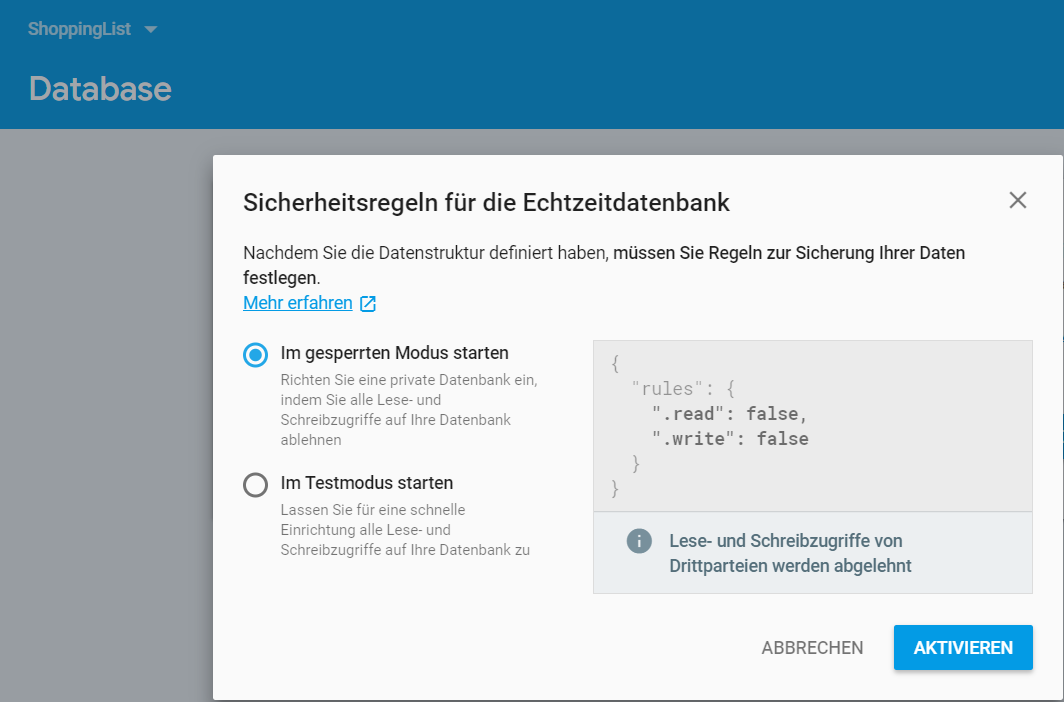
\includegraphics[width=0.7\linewidth]{images/RealtimeDBrules}
	\caption{Rules of RealtimeDB}
	\label{fig:realtimedbrules}
\end{figure}

\subsection{build.Gradle}
Nun werden die Projekt build.Gradle dependencys um folgende erweitert:
\begin{lstlisting}
classpath 'com.android.tools.build:gradle:3.0.1'
classpath 'com.google.gms:google-services:3.2.0'
classpath 'com.google.gms:google-services:3.0.0'
\end{lstlisting}

Das App build.Gradle File wird um folgendes erweitert:
\begin{lstlisting}
dependencies {
	implementation fileTree(dir: 'libs', include: ['*.jar'])
	implementation 'com.android.support:appcompat-v7:26.1.0'
	implementation 'com.android.support.constraint:constraint-layout:1.1.0'
	implementation 'com.android.support:design:26.1.0'
	testImplementation 'junit:junit:4.12'
	androidTestImplementation 'com.android.support.test:runner:1.0.1'
	androidTestImplementation 'com.android.support.test.espresso:espresso-core:3.0.1'
	compile fileTree(dir: 'libs', include: ['*.jar'])
	testCompile 'junit:junit:4.12'
	compile 'com.google.firebase:firebase-database:9.0.2'
}
apply plugin: 'com.google.gms.google-services'
\end{lstlisting}

\subsection{Internetzugriff}
Um der App Iternetzugriff zu gewähren wird im Manifest.xml File noch folgende Zeile hinzugefügt:
\begin{lstlisting}
<uses-permission android:name="android.permission.INTERNET"/>
\end{lstlisting}

\subsection{Strings.xml}
Außerdem muss im Strings.xml File (res/values/Strings.xml) folgende Ressource hinzugefügt werden um später Zugriff zu haben:
\begin{lstlisting}
<resources>
	<string name="app_name">ShoppingListApp</string>
	<string name="action_settings">Settings</string>
	<string name="add_task_button">Add Task</string>
</resources>
\end{lstlisting}

\subsection{Main Activity}
\subsubsection{Main Activity Layout}
Nun wird das Main Activity Layout File erstellt, dazu kann im Design Tab der Android Studios eine UI erstellt werden. Diese soll folgende Elemente aufweisen:
\begin{itemize}
	\item RecyclerView: Die View, in welcher später die ShoppingList Items angezeigt werden
	\item EditText: Ein Input-Feld um den Namen eines neuen Items einzugeben
	\item Button: Add Item Button um das Item hinzuzufügen
\end{itemize}

\begin{figure}[!h]
	\centering
	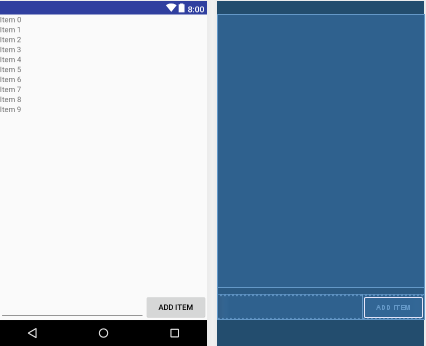
\includegraphics[width=0.6\linewidth]{images/layoutmain}
	\caption{Main Application UI}
	\label{fig:layoutmain}
\end{figure}

\subsubsection{Main Activity Java}
Die zugehörige Java Klasse \textit{MainActivity.java} bildet die Funktinonen der UI.

Beim klicken des Buttons wird der Inhalt des EditText Feldes gelesen und über die Push() und setValue() Methoden an die Datenbank gesendet. AUßerdem werden Items mit weniger als 6 Zeichen und Leere Items über eine Errormeldung abgefangen.

Hier der Code hinter der onClick() Methode desButtons:
\begin{lstlisting}[language=java]
addTaskButton.setOnClickListener(new View.OnClickListener() {
	@Override
	public void onClick(View view) {
		String enteredTask = addTaskBox.getText().toString();
		if(TextUtils.isEmpty(enteredTask)){
			Toast.makeText(MainActivity.this, "You must enter a task first", Toast.LENGTH_LONG).show();
		return;
	}
	if(enteredTask.length() < 6){
		Toast.makeText(MainActivity.this, "Task count must be more than 6", Toast.LENGTH_LONG).show();
		return;
	}
	Task taskObject = new Task(enteredTask);
	databaseReference.push().setValue(taskObject);
	addTaskBox.setText("");
	}
});
\end{lstlisting}

Danach wird ein ChildListener() Implementiert, welcher auf Veränderungen der Daten in der Firebase Datenbank reagiert. Falls also ein Item hinzugefügt wird oder verändert, wird durch die Methode \textit{getAllTask()} die Liste der Items aktualisiert. Falls ein Child entfernt wird wird über die Methode \textit{taskDeletion()} dieser entfernt.

\begin{lstlisting}[language=java]
databaseReference.addChildEventListener(new ChildEventListener() {
	@Override
	public void onChildAdded(DataSnapshot dataSnapshot, String s) {
		getAllTask(dataSnapshot);
	}
	@Override
	public void onChildChanged(DataSnapshot dataSnapshot, String s) {
		getAllTask(dataSnapshot);
	}
	@Override
	public void onChildRemoved(DataSnapshot dataSnapshot) {
		taskDeletion(dataSnapshot);
	}
});
\end{lstlisting}

Hier noch der Code der beiden Methoden \textit{getAllTask}:
\begin{lstlisting}[language=java]
private void getAllTask(DataSnapshot dataSnapshot){
	for(DataSnapshot singleSnapshot : dataSnapshot.getChildren()){
		String taskTitle = singleSnapshot.getValue(String.class);
		allTask.add(new Task(taskTitle));
		recyclerViewAdapter = new RecyclerViewAdapter(MainActivity.this, allTask);
		recyclerView.setAdapter(recyclerViewAdapter);
	}
}
\end{lstlisting}

\clearpage
und \textit{taskDeletion}:

\begin{lstlisting}[language=java]
private void taskDeletion(DataSnapshot dataSnapshot){
	for(DataSnapshot singleSnapshot : dataSnapshot.getChildren()) {
		String taskTitle = singleSnapshot.getValue(String.class);
		for(int i = 0; i < allTask.size(); i++){
			if(allTask.get(i).getTask().equals(taskTitle)){
			allTask.remove(i);
		}
	}
	Log.d(TAG, "Item tile " + taskTitle);
	recyclerViewAdapter.notifyDataSetChanged();
	recyclerViewAdapter = new RecyclerViewAdapter(MainActivity.this, allTask);
	recyclerView.setAdapter(recyclerViewAdapter);
}
\end{lstlisting}

\subsection{RecyclerView}
\subsubsection{RecyclerViewHolders.java}
Die RecyclerViewHolder Klasse fügt den Delete-Icons des einen Listener hinzu, welchen beim Drücken des Icons einen Toast (Flashmeldung) ausgibt und anschließend das Item, welches mit dem Icon verbunden ist aus der liste löscht.
\begin{lstlisting}[language=java]
deleteIcon.setOnClickListener(new View.OnClickListener() {
	@Override
	public void onClick(View v) {
		Toast.makeText(v.getContext(), "Delete icon has been clicked", Toast.LENGTH_LONG).show();
		String taskTitle = taskObject.get(getAdapterPosition()).getTask();
		Log.d(TAG, "Task Title " + taskTitle);
		DatabaseReference ref = FirebaseDatabase.getInstance().getReference();
		Query applesQuery = ref.orderByChild("task").equalTo(taskTitle);
		applesQuery.addListenerForSingleValueEvent(new ValueEventListener() {
			@Override
			public void onDataChange(DataSnapshot dataSnapshot) {
				for (DataSnapshot appleSnapshot: dataSnapshot.getChildren()) {
					appleSnapshot.getRef().removeValue();
				}
			}
			@Override
			public void onCancelled(DatabaseError databaseError) {
				Log.e(TAG, "onCancelled", databaseError.toException());
			}
		});
	}
});
\end{lstlisting}
\clearpage
\subsection{List View}
Anschließend wird eine View für die Item Liste erstellt. Diese enthält zuerst eine IMageView für das Shoppingcart Icon, eine TextView für den Namen des Items und eine ImageView für das Delete Icon zum Löschen des Items-Eintrags.

Diese sieht folgendermaßen aus:
\begin{figure}[!h]
	\centering
	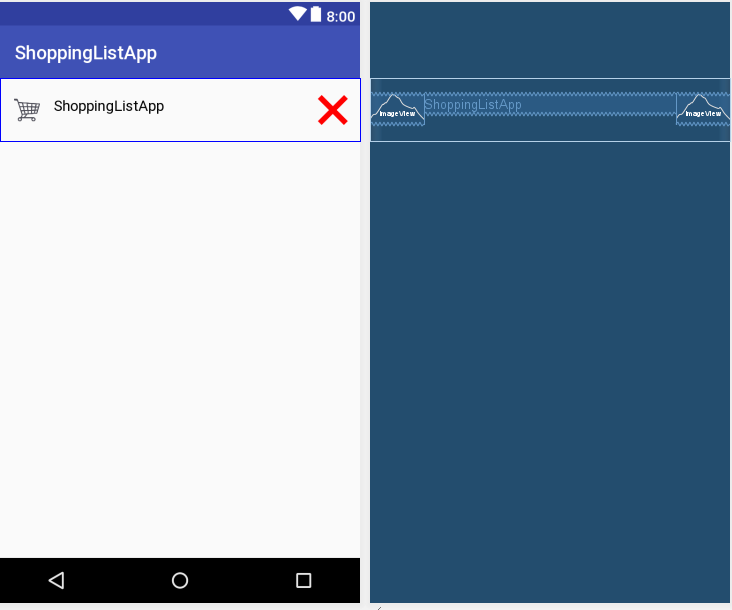
\includegraphics[width=0.6\linewidth]{images/listview}
	\caption{ListView}
	\label{fig:listview}
\end{figure}

xml-Code dazu:
\begin{lstlisting}
<ImageView
android:id="@+id/task_icon"
android:layout_width="0dp"
android:layout_height="32dp"
android:src="@mipmap/shoppingcart_front"
android:layout_weight="15"
android:contentDescription="@string/app_name" />
<TextView
android:id="@+id/task_title"
android:layout_width="0dp"
android:layout_height="wrap_content"
android:layout_weight="70"
android:text="@string/app_name"
android:textSize="16sp"
android:textColor="@color/colorBlack"/>

<ImageView
android:id="@+id/task_delete"
android:layout_width="0dp"
android:layout_height="32dp"
android:layout_weight="15"
android:contentDescription="@string/app_name"
android:src="@drawable/redx" />
\end{lstlisting}

\subsubsection{Custom Icons}
Um hier ein eigenes Icon einzufügen, muss man per Rechtsklick auf den ''res'' Ordner dann ''New'' -> ''Image Asset'' ein neues Asset hinzufügen. Ich habe hier ein Rotes X und ein Shoppingcart erstellt: 

\begin{figure} [!h]
	\subfigure[Rotes X Icon]{
\includegraphics[width=0.15\textwidth]{images/redx}} 
	\subfigure[Shoppingcart Icon]{
\includegraphics[width=0.15\textwidth]{images/shoppingcart}} 
	\caption{Verwendete Custom Icons} 
\end{figure} 

Daher auch der Aufruf per:
\begin{lstlisting}
adroid:src="@mipmap/shoppingcart_front" 
android:src="@mipmap/redx_front"
\end{lstlisting}

\subsection{Task}
Zuletzt wird noch eine Klasse für Task Objekte (Items) erstellt.

\begin{lstlisting}
public class Task {
	private String task;
	public Task() {}
	public Task(String task) {
		this.task = task;
	}
	public String getTask() {
		return task;
	}
}
\end{lstlisting}
\clearpage
\section{Ausführen}
\subsection{Emulator}
Somit ist die Implemetation fertig und die fertige App kann über den Vitual Device Viewer gestartet und getestet werden. Diese sieht dann nach 3 Einträgen folgendermaßen aus:
\begin{figure}[!h]
	\centering
	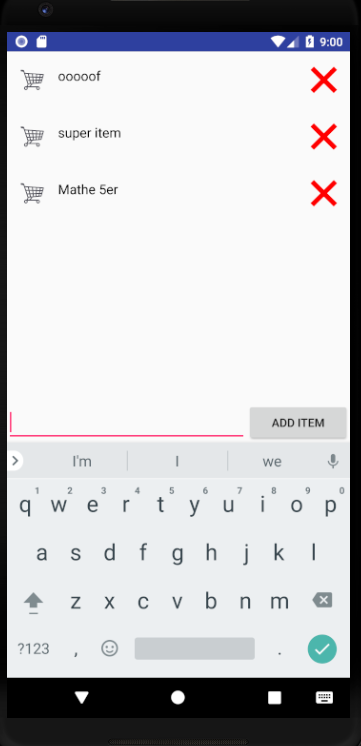
\includegraphics[width=0.27\linewidth]{images/runemulator}
	\caption{Emulator Screenshot}
	\label{fig:runemulator}
\end{figure}
\clearpage
\subsection{Firebase Konsole}
Nebenbei kann man in der Firebase Konsole die Änderungen am JSON File (also der Datenbank) mitverfolgen, hier wird pro Eintrag ein Key erstellt und unter diesem der in der TextEdit eingegeben Name für ein Item:
\begin{figure}[!h]
	\centering
	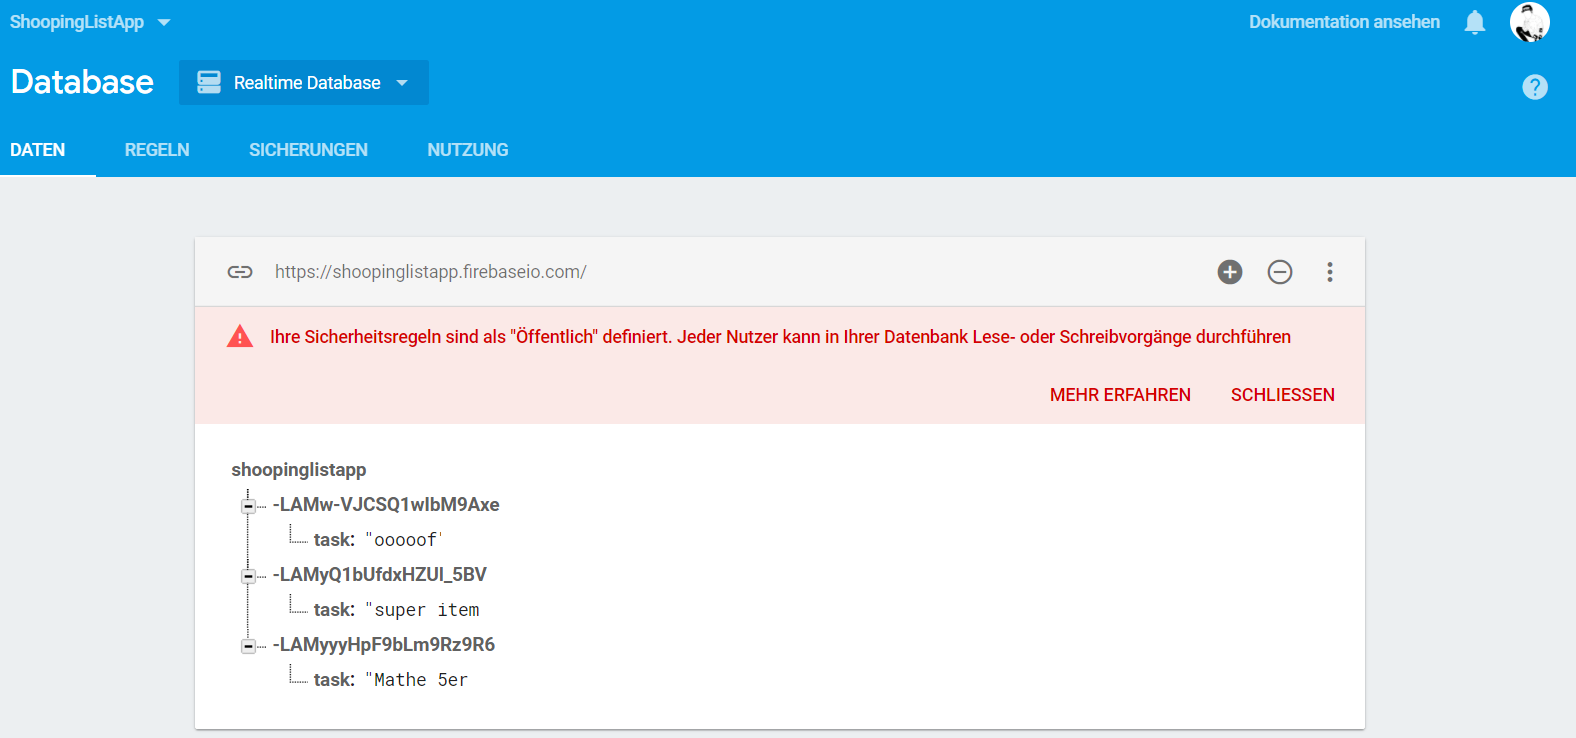
\includegraphics[width=0.9\linewidth]{images/firebaseconsole}
	\caption{Firebase Console}
	\label{fig:firebaseconsole}
\end{figure}

\subsection{APK}
Zuletzt kann man über Android Studio durch das Klicken von ''Build'' -> ''Build APKs'' eine APK der App erstellen und diese anschließend auf ein Android Handy laden. Ich habe diese auf mein Handy geladen und zusammen mit dem Emulator die Synchronität der Daten in der Liste überprüft. 

Wenn also am Handy ein Eintrag gelöscht wird, wird dieser auch im Emulator und in der Datenbank entfernt.




